\documentclass{article}%
\usepackage[T1]{fontenc}%
\usepackage[utf8]{inputenc}%
\usepackage{lmodern}%
\usepackage{textcomp}%
\usepackage{lastpage}%
\usepackage[head=40pt,margin=0.5in,bottom=0.6in]{geometry}%
\usepackage{graphicx}%
%
\title{\textbf{La oposición y el chavismo disidente se unen en defensa de la Constitución}}%
\author{RAFAEL LEÓN | raleon@el{-}nacional.com}%
\date{18/10/2018}%
%
\begin{document}%
\normalsize%
\maketitle%
\textbf{URL: }%
http://www.el{-}nacional.com/noticias/politica/oposicion{-}chavismo{-}disidente{-}unen{-}defensa{-}constitucion\_256240\newline%
%
\textbf{Periodico: }%
EN, %
ID: %
256240, %
Seccion: %
Política\newline%
%
\textbf{Palabras Claves: }%
Política, Oposición\newline%
%
\textbf{Derecho: }%
12%
, Otros Derechos: %
CONTEXTO%
, Sub Derechos: %
NO\_TIENE%
\newline%
%
\textbf{EP: }%
NO\newline%
\newline%
%
\textbf{\textit{Abogados y dirigentes advierten que el gobierno pretende “constitucionalizar” el modelo político que ha puesto en marcha la asamblea constituyente desde 2017}}%
\newline%
\newline%
%
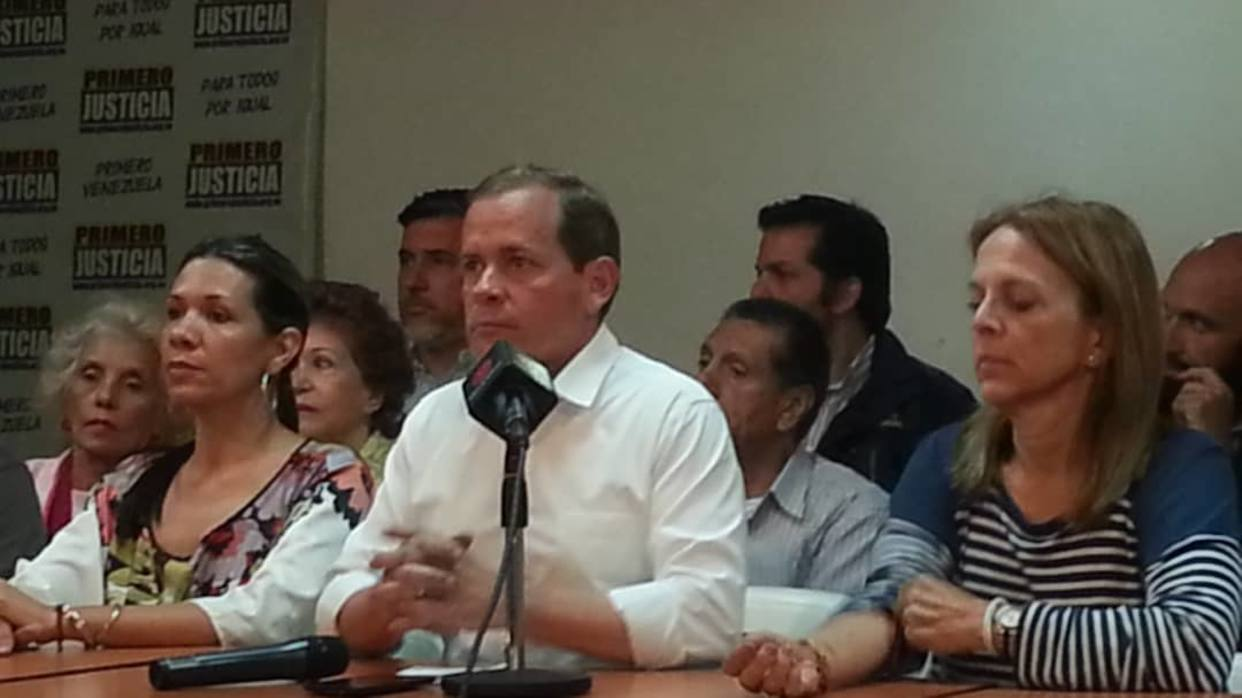
\includegraphics[width=300px]{98.jpg}%
\newline%
%
La amenaza de incluir en la Constitución el modelo político actual, que se instaura desde la asamblea nacional constituyente, ha generado puntos de encuentros entre sectores de la oposición y el chavismo disidente, que han sostenido reuniones en las últimas semanas para dar con una estrategia unitaria en defensa de la carta magna vigente desde 1999.%
\newline%
%
Negal Morales, secretario de la Asamblea Nacional e integrante del Frente Amplio Venezuela Libre, indicó que desde esta plataforma iniciaron una ronda de conversaciones para decidir si participan o se oponen a la modificación constitucional, y la enfrentan con movilización ante un posible referéndum.%
\newline%
%
El abogado constitucionalista Pedro Afonso del Pino indicó que ni en la Constitución ni en las bases comiciales está establecida la obligación de hacer un referéndum aprobatorio de una nueva carta magna. “La lógica constitucional y el precedente de 1999 lo obligarían, pero en la estrategia del gobierno no sé si esto está claro”, expresó. Recomendó a la oposición pensar en la participación en caso de que la aceptación del nuevo texto constitucional se someta a una consulta popular. “Esta huelga electoral nos lleva al salto al vacío”, advirtió.%
\newline%
%
“Si hay una movilización de todo el pueblo que permita estar en todas las mesas electorales, es posible derrotar al gobierno en las urnas, con unidad y sentido de la direccionalidad independientemente de la posición política”, manifestó Héctor Navarro, ex ministro de las carteras de Energía y Educación. Navarro considera que la defensa de la Constitución es un punto de partida para otras luchas que se podrían emprender por el bien común del país.%
\newline%
%
Morales exhortó a la Asamblea Nacional, que anunció la creación de una comisión en defensa de la Constitución, a integrar al equipo de trabajo al chavismo disidente y a los constituyentitas de 1999.%
\newline%
%
Navarro indicó que la ANC prepara una carta magna a discreción, sin discusión y bajo imposición. Afirmó que el hermetismo es tal, que hay constituyentes que desconocen el texto; incluso, la misma directiva de la ANC. “Ahora el siguiente paso que pretende dar el gobierno es aprobarla en unas condiciones que no sabemos, para formalizar la manera en que ellos han venido gobernando. Las versiones que han rodado echan a la borda las conquistas de la Constitución de~1999”, expresó.%
\newline%
%
Ilegalidad%
\newline%
%
Del Pino aseguró que en la práctica la constituyente ha estado haciendo una “Constitución dispersa” a través de varios textos normativos con rango constitucional, por ejemplo, cuando asume las competencias de la Asamblea Nacional o de otros poderes públicos.%
\newline%
%
Indicó que la constituyente es írrita desde su origen y que este año, que ha estado funcionado, ha ejecutado una violación integral de la Constitución, que incluyen el irrespeto a los artículos 7, 347, 348 y 349 que regulan la supremacía de los poderes y el funcionamiento de una asamblea constituyente.%
\newline%
%
“Hay dudas si realmente el interés del gobierno es hacer una nueva Constitución o mantener la ANC que sirve de salvavidas para ‘legalizar’ los actos que están fuera de la carta magna”, añadió Del Pino.%
\newline%
%
Al igual que Navarro y la ONG Acceso a la Justicia, Del Pino advirtió que desde la ANC se pretende dar rango constitucional al modelo político que se ha puesto en marcha desde julio del año pasado, en el que se viola continuamente la carta magna. De acuerdo con Acceso a la Justicia, el borrador del texto que se redacta desde la ANC, establece cambios radicales en la Constitución, entre ellos el desmantelamiento del Estado federal por el llamado Estado comunal, limitación importante de la propiedad privada y “constitucionalización” –darle rango constitucional– de la propiedad social y propiedad colectiva, así como la supresión de la independencia de los Poderes Públicos y la inclusión de delito de traición a la patria.%
\newline%
%
María Corina Machado, coordinadora de Vente Venezuela, alertó que el gobierno negocia la imposición de la carta magna que se redacta en la ANC, ofreciendo a cambio la renovación de Poderes Públicos en dos años.%
\newline%
%
“Dos años más de Maduro en el poder, a cambio de que se juramente en la AN legítima el 10 de enero con el voto favorable no solamente con los diputados del PSUV, sino algunos que se llaman oposición”, explicó desde la Embajada de España, donde consignó un documento en rechazo del diálogo.%
\newline%
%
El Dato%
\newline%
%
El Frente Amplio Venezuela Libre prepara un congreso que se desarrollará en el mes de noviembre, informó Negal Morales. A través de las actividades, la dirigencia busca escuchar la voz de los opositores en las regiones del país para luego elevarlo a un congreso nacional. Dijo que el objetivo es lograr la unión de los venezolanos y una estrategia de lucha para evitar “la imposición de una nueva Constitución”.%
\newline%
%
\end{document}